%% LyX 2.3.6 created this file.  For more info, see http://www.lyx.org/.
%% Do not edit unless you really know what you are doing.
\documentclass[english]{article}
\usepackage[T1]{fontenc}
\usepackage[latin9]{inputenc}
\usepackage{geometry}
\geometry{verbose,tmargin=3cm,bmargin=3cm,lmargin=3cm,rmargin=3cm}
\usepackage{array}
\usepackage{fancybox}
\usepackage{calc}
\usepackage{multirow}
\usepackage{amsmath}
\usepackage{amsthm}
\usepackage{amssymb}
\usepackage{graphicx}
\usepackage{setspace}
\onehalfspacing

\makeatletter

%%%%%%%%%%%%%%%%%%%%%%%%%%%%%% LyX specific LaTeX commands.
%% Because html converters don't know tabularnewline
\providecommand{\tabularnewline}{\\}

%%%%%%%%%%%%%%%%%%%%%%%%%%%%%% Textclass specific LaTeX commands.
\theoremstyle{plain}
\newtheorem{thm}{\protect\theoremname}
\theoremstyle{definition}
\newtheorem{xca}[thm]{\protect\exercisename}
\theoremstyle{remark}
\newtheorem*{rem*}{\protect\remarkname}
\theoremstyle{remark}
\newtheorem*{conclusion*}{\protect\conclusionname}

%%%%%%%%%%%%%%%%%%%%%%%%%%%%%% User specified LaTeX commands.
\DeclareMathOperator*{\argmin}{argmin}
\DeclareMathOperator*{\argmax}{argmax}

\@ifundefined{showcaptionsetup}{}{%
 \PassOptionsToPackage{caption=false}{subfig}}
\usepackage{subfig}
\makeatother

\usepackage{babel}
\usepackage{listings}
\providecommand{\conclusionname}{Conclusion}
\providecommand{\exercisename}{Exercise}
\providecommand{\remarkname}{Remark}
\providecommand{\theoremname}{Theorem}
\renewcommand{\lstlistingname}{Listing}

\begin{document}
\title{Compressed Sensing -- Sheet 12}
\author{Ferdinand Vanmaele}
\maketitle
\begin{xca}[Programming project part 1]
\mbox{}
\begin{itemize}
\item The generation of sensors is done in \texttt{sheet12\_ex1/sensors.py}.
To make the matrices work with the assumptions of CoSaMP, OMP, SP
and MP as defined in the lecture, the columns are normalized.
\begin{itemize}
\item $m$ rows are drawn uniformly at random (without repetition) by generating
a random permutation $S(m)\rightarrow S(m)$.
\end{itemize}
\item Random $s$-sparse vectors $x\in\mathbb{R}^{n}$ with $1\leq s\leq m$
are constructed in \texttt{sheet12\_ex1/main.py}. The \texttt{generate\_problems()}
function takes the problem dimension $n$ and bounds for $s$, as
well as the number repetitions for each sparsity value.
\item Algorithms are run in \texttt{sheet12\_ex1/main.py}. Every algorithm
is implemented in its own function\footnote{This is a bit repetitive, especially for closely related algorithms
such as CoSaMP and SP. However, every different algorithm to be tested
is self-contained in this way. Outside of this exercise, I would likely
summarize some functions and add additional parameters.} and can be enabled or disabled selectively.

\noindent\shadowbox{\begin{minipage}[t]{1\columnwidth - 2\fboxsep - 2\fboxrule - \shadowsize}%
\begin{rem*}
The following modifications were made:
\begin{itemize}
\item A tolerance of $10^{-8}$ was chosen te reduce oscillations for different
sparsity levels.
\item Iterative hard thresholding was implemented with a variable step size
{[}TBDR12{]}, 
\[
g:=A^{\ast}r^{(k)},\quad T:=\begin{cases}
\text{supp}(\mathcal{T}(g,s)) & \text{if }k>0\\
\text{supp}(\mathcal{T}(x^{(0)},s)) & \text{if }k=0
\end{cases},\quad\mu:=\frac{\|g_{T}\|_{2}^{2}}{\|A_{T}g_{T}\|_{2}^{2}}
\]
instead of $\mu=1$. In the experiments performed, this was done to
avoid divergence with $\mu=1$.
\end{itemize}
\end{rem*}
%
\end{minipage}}
\item Let $\text{RE}(\hat{x}):=\|x-\hat{x}\|_{2}/\|x\|_{2}$. We consider
successful recovery of a vector of sparsity $1\leq s\leq m$ as the
maximum $s$, such that
\[
s_{\max}:=\max_{s}\left\{ \forall s'\leq s:\,\frac{1}{100}\sum_{i\in[100]}\text{RE}(\hat{x}_{s',i})<10^{-6}\right\} 
\]
holds. Summary of the trials, with $n=128$, $m=2^{7}$:
\begin{center}
\begin{tabular}{|c|c|c|c|c|}
\hline 
Matrix &  & Algorithm & $s_{\max}$ & $\approx\sum\text{RE}$\tabularnewline
\hline 
\hline 
\multirow{8}{*}{\textbf{Random }($A$)} & 1 & $\ell_{1}$-min. (BP) & $s=17$ & $10^{-9}$\tabularnewline
\cline{2-5} \cline{3-5} \cline{4-5} \cline{5-5} 
 & 2 & OMP & $s=13$ & $10^{-15}$\tabularnewline
\cline{2-5} \cline{3-5} \cline{4-5} \cline{5-5} 
 & 3 & MP & $s=5$ & $10^{-9}$\tabularnewline
\cline{2-5} \cline{3-5} \cline{4-5} \cline{5-5} 
 & 4 & IHT & $s=10$ & $10^{-9}$\tabularnewline
\cline{2-5} \cline{3-5} \cline{4-5} \cline{5-5} 
 & 5 & CoSaMP & $s=14$ & $10^{-15}$\tabularnewline
\cline{2-5} \cline{3-5} \cline{4-5} \cline{5-5} 
 & 6 & BT & $s=0$ & $-$\tabularnewline
\cline{2-5} \cline{3-5} \cline{4-5} \cline{5-5} 
 & 7 & HTP & $s=10$ & $10^{-15}$\tabularnewline
\cline{2-5} \cline{3-5} \cline{4-5} \cline{5-5} 
 & 8 & SP & $s=15$ & $10^{-15}$\tabularnewline
\hline 
\multirow{8}{*}{\textbf{Fourier }($F$)} & 1 & $\ell_{1}$-min. (BP) & $s=40$ & $10^{-10}$\tabularnewline
\cline{2-5} \cline{3-5} \cline{4-5} \cline{5-5} 
 & 2 & OMP & $s=34$ & $10^{-15}$\tabularnewline
\cline{2-5} \cline{3-5} \cline{4-5} \cline{5-5} 
 & 3 & MP & $s=10$ & $10^{-7}$\tabularnewline
\cline{2-5} \cline{3-5} \cline{4-5} \cline{5-5} 
 & 4 & IHT & $s=26$ & $10^{-9}$\tabularnewline
\cline{2-5} \cline{3-5} \cline{4-5} \cline{5-5} 
 & 5 & CoSaMP & $s=25$ & $10^{-15}$\tabularnewline
\cline{2-5} \cline{3-5} \cline{4-5} \cline{5-5} 
 & 6 & BT & $s=0$ & $-$\tabularnewline
\cline{2-5} \cline{3-5} \cline{4-5} \cline{5-5} 
 & 7 & HTP & $s=26$ & $10^{-15}$\tabularnewline
\cline{2-5} \cline{3-5} \cline{4-5} \cline{5-5} 
 & 8 & SP & $s=31$ & $10^{-15}$\tabularnewline
\hline 
\end{tabular}
\par\end{center}
\item Conclusions:
\begin{itemize}
\item Methods using orthogonal projection recover the solution at a high
accuracy (close to machine precision) for $1\leq s$ sufficiently
small. IHT is still competitive in terms of $s_{\max}$, with a higher
recovery level.
\item The recovery error increased steeply from $s_{\max}$ to higher levels
$s>s_{\max}$. Some trials also had oscillatory behavior.
\item The Fourier matrix was recovered for higher sparsity levels for all
algorithms except Basic Thresholding. The coherence of this matrix
is much lower than the Gaussian one ($\approx0.08$ vs. $\approx1.00$)
so this is unsurprising.
\item $\ell_{1}$-minimization had constant performance for all trials.
Methods using orthogonal projection had their CPU time increase exponentially.
(See Figure \ref{fig:Combined-CPU-time-Gaussian} and \ref{fig:Combined-CPU-time-Fourier})
\end{itemize}
\end{itemize}
\end{xca}

\begin{figure}[h]
\begin{centering}
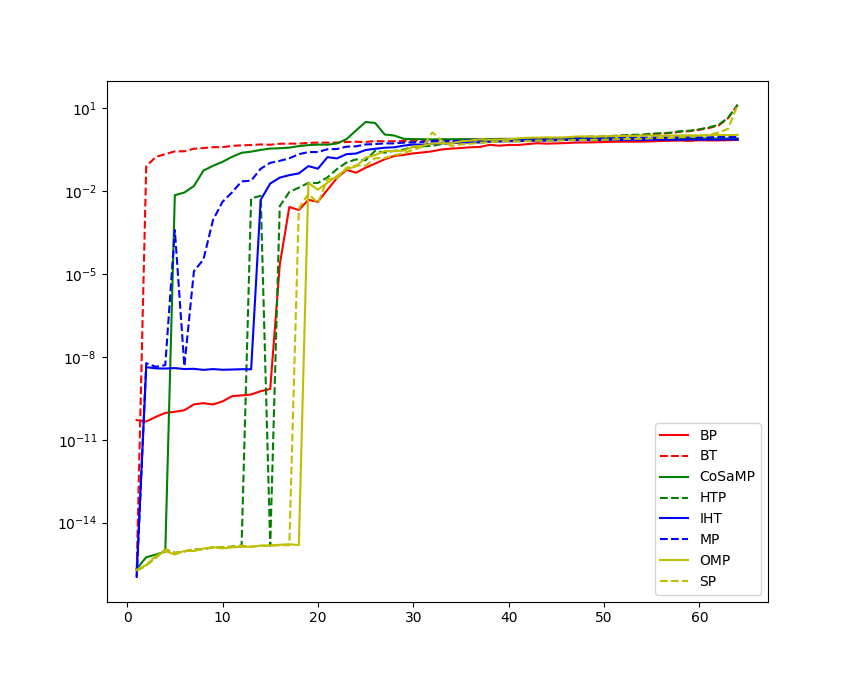
\includegraphics[width=0.9\columnwidth]{A_m64_n128_100_error}
\par\end{centering}
\caption{Relative recovery error ($y$-axis) over 100 trials per sparsity $1\protect\leq s\protect\leq m$
($x$-axis) for \textbf{Gaussian} \textbf{matrix} $A\in\mathbb{R}^{64\times128}$
with normalized columns.\label{fig:Relative-recovery-error-Gaussian}}
\end{figure}

\begin{figure}[h]
\begin{centering}
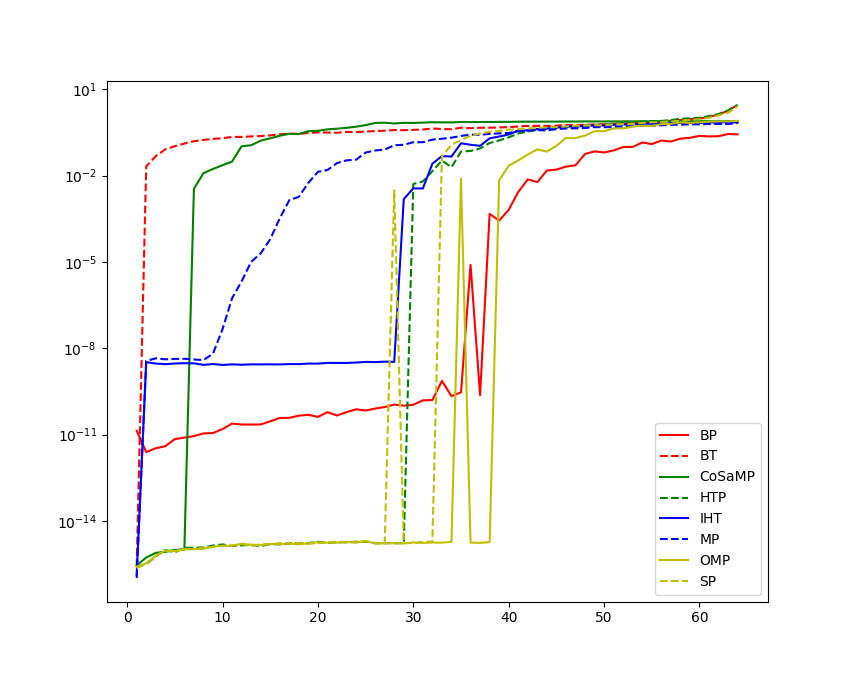
\includegraphics[width=0.8\columnwidth]{F_m64_n128_100_error}
\par\end{centering}
\caption{Relative recovery error ($y$-axis) averaged over 100 trials, by sparsity
level $1\protect\leq s\protect\leq m$ ($x$-axis) for \textbf{partial
Fourier} \textbf{matrix} $F\in\mathbb{R}^{64\times128}$ with normalized
columns.\label{fig:Relative-recovery-error-Fourier}}
\end{figure}

\begin{figure}[h]
\begin{centering}
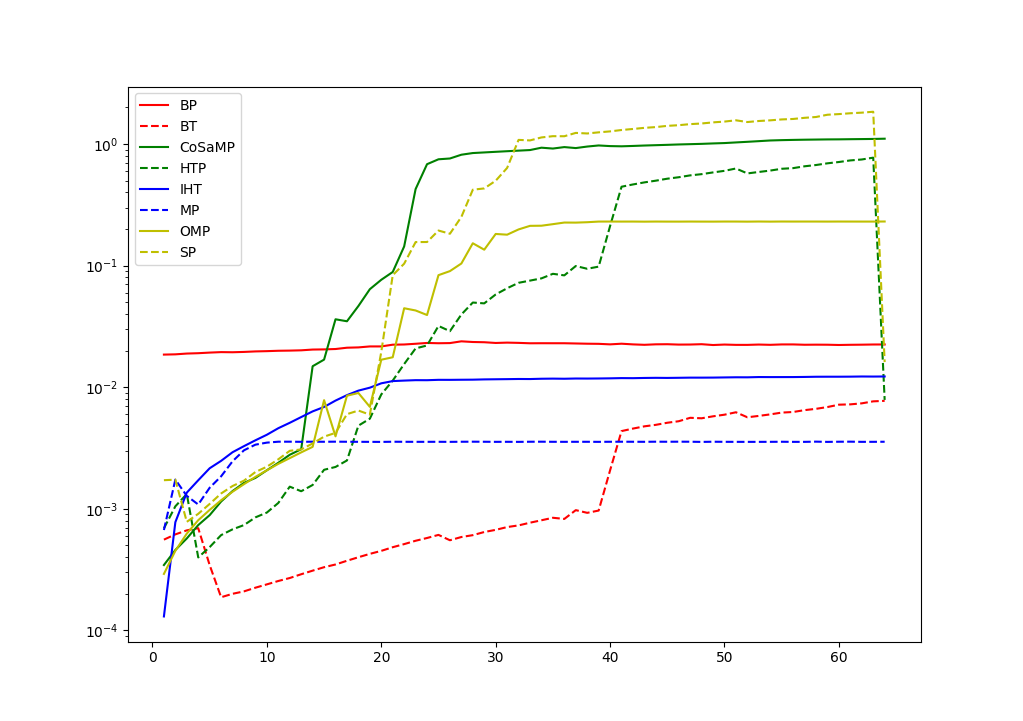
\includegraphics[width=0.8\columnwidth]{A_m64_n128_100_cputime}
\par\end{centering}
\caption{Combined CPU time in seconds per iteration ($y$-axis) averaged over
100 trials, by sparsity level $1\protect\leq s\protect\leq m$ for
\textbf{Gaussian matrix} $A\in\mathbb{R}^{64\times128}$ with normalized
columns.\label{fig:Combined-CPU-time-Gaussian}}

\end{figure}

\begin{figure}[h]
\begin{centering}
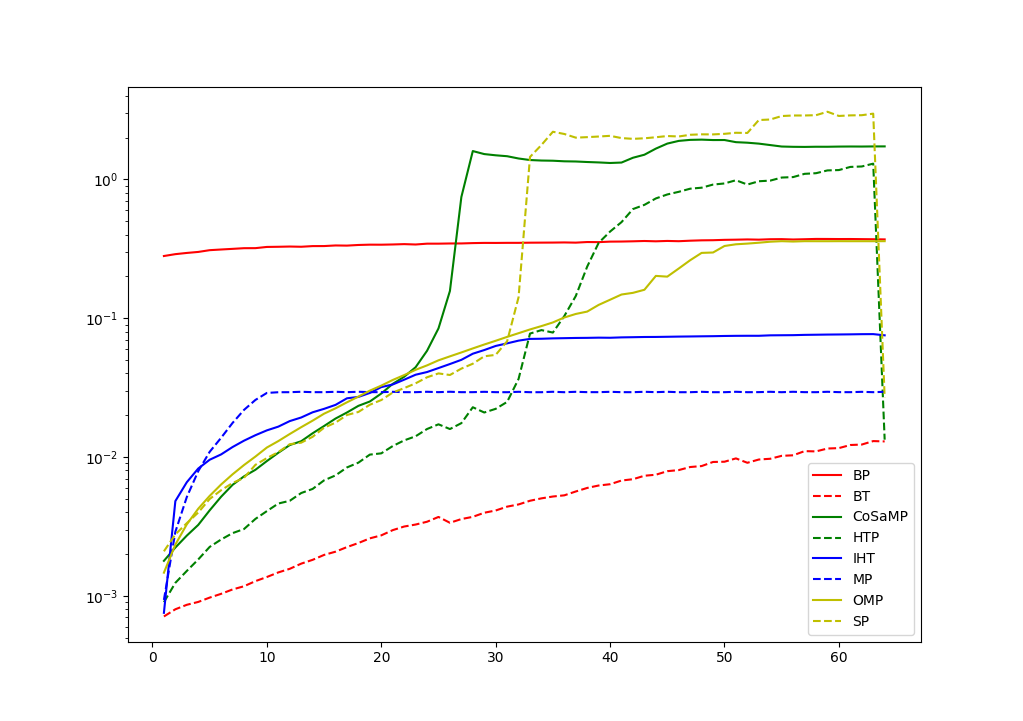
\includegraphics[width=0.8\columnwidth]{F_m64_n128_100_cputime}
\par\end{centering}
\caption{Combined CPU time in seconds per iteration ($y$-axis) averaged over
100 trials, by sparsity level $1\protect\leq s\protect\leq m$ for
\textbf{partial Fourier matrix} $F\in\mathbb{R}^{64\times128}$ with
normalized columns.\label{fig:Combined-CPU-time-Fourier}}

\end{figure}

\newpage{}
\begin{xca}
\mbox{}
\end{xca}


\subsection*{Problem definition}

The robust face recognition problem is given by
\[
\min_{w\in\mathbb{R}^{m+n}}\frac{1}{2}\|Bw-b\|_{2}^{2}+\lambda\|w\|_{1}
\]
where
\begin{itemize}
\item $\lambda\in\mathbb{R}_{>0}$ is a regularization parameter, 
\begin{itemize}
\item $B=[A\quad I]\in\mathbb{R}^{m\times(m+n)}$ with $A\in\mathbb{R}^{m\times n}$,
$I\in\mathbb{R}^{m\times m}$ a highly correlated dictionary of $m$
face images $v\in\mathbb{R}^{n}$, stacked column-wise;
\item $I$ the identity matrix $\in\mathbb{R}^{n\times n}$, $b=Ax+e$ a
face image to be recognized not in the dictionary $A$, with $e\in\mathbb{R}^{n}$
an unknown error;
\item $w$ the minimization variable. 
\end{itemize}
The term $F(w):=\frac{1}{2}\|Bw-b\|_{2}^{2}$ is differentiable,
\begin{equation}
\nabla F(w)=B^{T}(Bw-b)\label{eq:minimization}
\end{equation}
with Lipschitz constant $L:=\|B^{T}B\|_{F}$,
\begin{align*}
\|B^{T}(Bw-b)-B^{T}(Bz-b)\|_{2} & =\|B^{T}Bw-B^{T}b-B^{T}Bz+B^{T}b\|_{2}\\
 & =\|B^{T}Bw-B^{T}Bz\|_{2}\\
 & \leq\|B^{T}B\|_{F}\|w-z\|_{2}.
\end{align*}
The norm $\|w\|_{1}$ is proper, convex and lsc and has as proximal
operator \textbf{soft shrinkage}, given component-wise by
\[
\left[\text{Prox}_{\gamma\|\cdot\|}(w)\right]_{i}=\begin{cases}
w_{i}+\gamma & \text{if }w_{i}<\gamma,\\
0 & \text{if }-\gamma\leq w_{i}\leq\gamma,\\
w_{i}-\gamma & \text{if }w_{i}>\gamma.
\end{cases}
\]
Multiplying by $\lambda>0$ we have:
\begin{align*}
\left[\text{Prox}_{\gamma R}(w)\right]_{i} & =\lambda^{-1}\left[\text{Prox}_{\lambda^{2}\gamma\|\cdot\|}(\lambda w)\right]_{i}\\
 & =\begin{cases}
w_{i}+\lambda\gamma & \text{if }w_{i}<\lambda\gamma,\\
0 & \text{if }-\lambda\gamma\leq w_{i}\leq\lambda\gamma,\\
w_{i}-\lambda\gamma & \text{if }w_{i}>\lambda\gamma.
\end{cases}
\end{align*}

The non-zero entries of $x_{\ast}$ in the solution $w_{\ast}=[x_{\ast}^{T},e_{\ast}^{T}]^{T}$
of problem (\ref{eq:minimization}) represent the person the image
belongs to.
\begin{rem*}
When we consider images without noise, we have the optimization problem
\begin{equation}
\min_{x\in\mathbb{R}^{m}}\frac{1}{2}\|Ax-b\|_{2}^{2}+\lambda\|x\|_{1}\label{eq:basis-pursuit}
\end{equation}
with gradient $\nabla F(w)=A^{T}(Ax-b)$ and proximal operator as
above. The non-zero entries of the solution $x_{\ast}$ represent
the person the image belongs to. In pratice this can only hold approximately,
and we look instead at the vector 
\[
|x|_{\downarrow}=(|x|_{[1]},|x|_{[2]},\dots),\quad|x|_{[1]}\geq|x|_{[2]}\geq\cdots
\]
 of sorted by absolute magnitude of its elements.
\end{rem*}
\end{itemize}

\subsection*{Face recognition data set}

We assemble the dictionary $A$ as follows. The baseline is the \emph{Labeled
Faces in the Wild}\footnote{https://www.kaggle.com/datasets/jessicali9530/lfw-dataset}
(LFW) dataset, with each image of size $(250,250)$. Images in this
dataset are aligned, but not cropped so that background details (and
potentially multiple faces) are visible. In a first attempt, $A$
is constructed by randomly selecting 508 persons from this dataset
which have at least 5 images available. Then, 4 images are selected
randomly to construct A (training set), and 1 image is selected randomly
for the complement for the reconstruction (verification set).

\begin{lstlisting}[language=Python,numbers=left,numberstyle={\scriptsize},basicstyle={\small},breaklines=true,tabsize=4,frame=simple]
for person in people:
    # reduce number of people in data set for performance reasons
    dice_roll = np.random.choice([1,2,3,4,5,6])
    if dice_roll == 1 or dice_roll == 3:
        idx = people[person]
    
        if len(idx) >= min_samples:
            idx_train = np.random.choice(idx, num_train)
            idx_verif = np.random.choice(np.setdiff1d(idx, idx_train), num_verif)

            training_set[person] = idx_train
            verification_set[person] = idx_verif
\end{lstlisting}

The parameters for FISTA-Mod were chosen as follows: 
\begin{itemize}
\item $\lambda=10^{-3}$ and $x_{0}=0\in\mathbb{R}^{n+m}$;
\item $TOL=10^{-7}$ where the algorithm terminates if $\|x^{(k-1)}-x^{(k)}\|<TOL$
or 5000 iterations were exceeded.
\item $p=\frac{1}{20}$, $q=\frac{1}{2}$, $r=4$.
\end{itemize}
For recognizing original images (that is, images with no noise added),
FISTA-Mod applied to problem (\ref{eq:basis-pursuit}) could not uniquely
recover a sample from the verification set, even though the sequence
$\{x^{(k)}\}$ converged. See Figure \ref{fig:uncropped-results}.
The cause was likely images having more than a single face available
or other background artifacts. See Figure \ref{fig:uncropped-results}
and \ref{fig:convergence-uncropped}.

\begin{figure}[h]
\hfill{}%
\begin{minipage}[b][1\totalheight][t]{0.2\columnwidth}%
\begin{center}
\subfloat[Original]{\begin{centering}
\includegraphics[width=1\columnwidth]{\string"/home/fvanmaele/source/repos/fista-mod/sheet12_ex2/Figure 2022-11-07 222229\string".png}
\par\end{centering}
}
\par\end{center}%
\end{minipage}\hfill{}%
\begin{minipage}[t]{0.2\columnwidth}%
\subfloat[$Bx^{\ast}$]{\begin{centering}
\includegraphics[width=1\columnwidth]{\string"/home/fvanmaele/source/repos/fista-mod/sheet12_ex2/Figure 2022-11-07 222319\string".png}
\par\end{centering}
}%
\end{minipage}\hfill{}%
\begin{minipage}[t]{0.2\columnwidth}%
\subfloat[{$B_{|x^{\ast}|_{[1]}}$}]{\begin{centering}
\includegraphics[width=1\columnwidth]{\string"/home/fvanmaele/source/repos/fista-mod/sheet12_ex2/Figure 2022-11-07 222323\string".png}
\par\end{centering}
}%
\end{minipage}\hfill{}%
\begin{minipage}[t]{0.2\columnwidth}%
\subfloat[{$B_{|x^{\ast}|_{[2]}}$}]{\includegraphics[width=1\columnwidth]{\string"/home/fvanmaele/source/repos/fista-mod/sheet12_ex2/Figure 2022-11-07 222328\string".png}

}%
\end{minipage}\hfill{}%
\begin{minipage}[t]{0.2\columnwidth}%
\subfloat[{$B_{|x^{\ast}|_{[3]}}$}]{\includegraphics[width=1\columnwidth]{\string"/home/fvanmaele/source/repos/fista-mod/sheet12_ex2/Figure 2022-11-07 222331\string".png}

}%
\end{minipage}

\caption{Recovered images for uncropped 250x250 sample\label{fig:uncropped-results}}

\end{figure}

\begin{figure}[h]
\hfill{}%
\begin{minipage}[t]{0.5\columnwidth}%
\subfloat[Values of $x^{\ast}$]{\begin{centering}
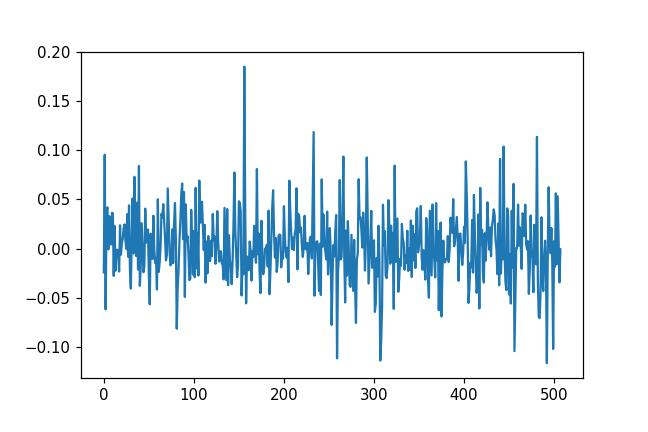
\includegraphics[width=1\columnwidth]{/home/fvanmaele/source/repos/fista-mod/sheet12_ex2/fista_mod_uncropped}
\par\end{centering}

}%
\end{minipage}\hfill{}%
\begin{minipage}[t]{0.5\columnwidth}%
\subfloat[Differences $J(x^{(k)})-J(x^{(k-1)})$ and $\|x^{(k)}-x^{(k-1)}\|$
by number of iterations]{\begin{centering}
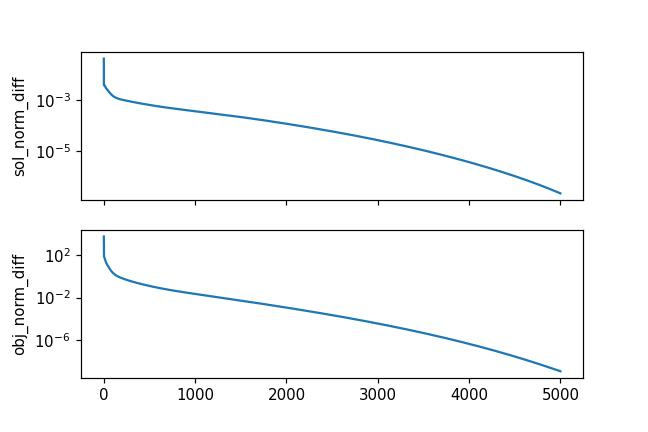
\includegraphics[width=1\columnwidth]{/home/fvanmaele/source/repos/fista-mod/sheet12_ex2/fista_mod_uncropped_norm_diff}
\par\end{centering}

}%
\end{minipage}

\caption{Convergence and values of $x^{\ast}$ for uncropped 250x250 sample
and $\lambda=10^{-3}$\label{fig:convergence-uncropped}}

\end{figure}

To address this, the images were cropped to regions containing a face
using cascade classifiers.\footnote{https://docs.opencv.org/3.4/db/d28/tutorial\_cascade\_classifier.html}
Since the resulting images had different sizes, all samples below
100 pixels and above 130 pixels height and width were removed. The
rest were then resized to 130 pixels height and width. The final training
set contained 776 images, so that $A\in\mathbb{R}^{16900\times776}$,
and an image from the verification set containing 245 items was selected.
This time around, the algorithm managed to recognize the person belonging
to given sample $b$. The parameter $\lambda$ was increased to $\lambda=1$,
and the tolerance lowered to $TOL=10^{-4}$ with a maximum of 5000
iterations. See Figure \ref{fig:cropped-results} and \ref{fig:convergence-cropped}.

\begin{figure}[h]
\hfill{}%
\begin{minipage}[b][1\totalheight][t]{0.2\columnwidth}%
\begin{center}
\subfloat[Original]{\begin{centering}
\includegraphics[width=1\columnwidth]{\string"/home/fvanmaele/source/repos/fista-mod/sheet12_ex2/Figure 2022-11-08 015303\string".png}
\par\end{centering}
}
\par\end{center}%
\end{minipage}\hfill{}%
\begin{minipage}[t]{0.2\columnwidth}%
\subfloat[$Bx^{\ast}$]{\begin{centering}
\includegraphics[width=1\columnwidth]{\string"/home/fvanmaele/source/repos/fista-mod/sheet12_ex2/Figure 2022-11-08 015802\string".png}
\par\end{centering}
}%
\end{minipage}\hfill{}%
\begin{minipage}[t]{0.2\columnwidth}%
\subfloat[{$B_{|x^{\ast}|_{[1]}}$}]{\begin{centering}
\includegraphics[width=1\columnwidth]{\string"/home/fvanmaele/source/repos/fista-mod/sheet12_ex2/Figure 2022-11-08 015511\string".png}
\par\end{centering}
}%
\end{minipage}\hfill{}%
\begin{minipage}[t]{0.2\columnwidth}%
\subfloat[{$B_{|x^{\ast}|_{[2]}}$}]{\includegraphics[width=1\columnwidth]{\string"/home/fvanmaele/source/repos/fista-mod/sheet12_ex2/Figure 2022-11-08 015514\string".png}

}%
\end{minipage}\hfill{}%
\begin{minipage}[t]{0.2\columnwidth}%
\subfloat[{$B_{|x^{\ast}|_{[3]}}$}]{\includegraphics[width=1\columnwidth]{\string"/home/fvanmaele/source/repos/fista-mod/sheet12_ex2/Figure 2022-11-08 015518\string".png}

}%
\end{minipage}

\caption{Recovered images for cropped 130x130 sample and $\lambda=1$ \label{fig:cropped-results}}
\end{figure}

\begin{figure}[h]
\hfill{}%
\begin{minipage}[t]{0.5\columnwidth}%
\subfloat[Values of $x^{\ast}$]{\begin{centering}
\includegraphics[width=1\columnwidth]{\string"/home/fvanmaele/source/repos/fista-mod/sheet12_ex2/Figure 2022-11-08 015440\string".png}
\par\end{centering}
}%
\end{minipage}\hfill{}%
\begin{minipage}[t]{0.5\columnwidth}%
\subfloat[Differences $J(x^{(k)})-J(x^{(k-1)})$ and $\|x^{(k)}-x^{(k-1)}\|$
by number of iterations]{\begin{centering}
\includegraphics[width=1\columnwidth]{\string"/home/fvanmaele/source/repos/fista-mod/sheet12_ex2/Figure 2022-11-08 020308\string".png}
\par\end{centering}
}%
\end{minipage}

\caption{Convergence and values of $x^{\ast}$ for cropped 130x130 sample and
$\lambda=1$\label{fig:convergence-cropped}}
\end{figure}

\begin{conclusion*}
FISTA-Mod applied to the face recognition problem managed to recognize
a sample, provided a clear image of the same person is available in
the dictionary $A$ is available. ``Clear image'' implies a fair
amount of preprocessing required: alignment (``funneling'') as provided
by the LFW dataset, and cropping with cascade classifiers so that
background details are not considered.
\end{conclusion*}

\end{document}
